\documentclass{article}
\usepackage[margin=1in]{geometry}      % default margins are too big
\usepackage{graphicx}                  % for \includegraphics
\usepackage{listings}                  % for typesetting source code
\lstset{language=Python}
\usepackage{mathtools}                 % for better typesetting of math
%\usepackage[round]{natbib}                    % for using different bibliography styles
\bibliographystyle{ieeetr}  
\usepackage{url}
%\usepackage{amsmath}

\usepackage{caption}
\usepackage{subcaption}
\usepackage{listings}
\usepackage{color}

\definecolor{dkgreen}{rgb}{0,0.6,0}
\definecolor{gray}{rgb}{0.5,0.5,0.5}
\definecolor{mauve}{rgb}{0.58,0,0.82}

\lstset{frame=tb,
  language=Java,
  aboveskip=3mm,
  belowskip=3mm,
  showstringspaces=false,
  columns=flexible,
  basicstyle={\small\ttfamily},
  numbers=none,
  numberstyle=\tiny\color{gray},
  keywordstyle=\color{blue},
  commentstyle=\color{dkgreen},
  stringstyle=\color{mauve},
  breaklines=true,
  breakatwhitespace=true
  tabsize=3
}                 % for typesetting source code

\begin{document}

\title{Project Report\\
Machine Learning techniques for\\
Offloading Smartphone Computing on Cloud to Save battery Power}
\author{Aditya Khune}
\date{\today}  % Leave this line out to use the current date.
\maketitle

%%%%%%%%%%%%%%%%%%%%%%%%%%%%%%%%%%%%%%%%%%%%%%%%%%%%%%%%%%%%%%%%%%%%%%

\tableofcontents

%%%%%%%%%%%%%%%%%%%%%%%%%%%%%%%%%%%%%%%%%%%%%%%%%%%%%%%%%%%%%%%%%%%%%%

\begin{abstract}
Smartphones have become the primary computing platform for many users. Various studies have identified longer battery lifetime as the most desired
feature of such systems. Low-power design has been an active research topic for
many years. Some studies such as in \cite{kumar2010cloud} suggest that many applications are too computation and if offloaded on the cloud then can
actually save battery power.\par
In this project I have studied this solution of offloading the computing on the cloud. After studying the problem I have proposed a decision engine based on some machine learning techniques which will act as an enhancement to the offloading process. In \cite{flores2013adaptive} authors have suggested a similar decision engine based on fuzzy logic. I have implemented a similar decision engine to start with and then used Reinforcement learning to take the right decision of whether to offload or not.
\end{abstract}

%%%%%%%%%%%%%%%%%%%%%%%%%%%%%%%%%%%%%%%%%%%%%%%%%%%%%%%%%%%%%%%%%%%%%%

\section{Introduction}
Mobile cloud computing is arising as a prominent domain
that is seeking to bring the massive advantages of the cloud
to the resource constrained smartphones. 
Offloading Smartphone Computing on Cloud is a technique that allows to empower the computational capabilities
of mobiles with cloud resources. Code offloading refers to a technique, in which resource intensive mobile components are identified and offloaded to remote processing in order to be executed by cloud-based surrogates. Most of the prominent works in the domain have proposed solutions to overcome the issues related with deciding whether to offload or
not to cloud.
%%%%%%%%%%%%%%%%%%%%%%%%%%%%%%%%%%%%%%%
\subsection{Offloading computation to save energy}
Cloud vendors provide computing cycles, and users
can use these cycles to reduce the amounts of computation
on mobile systems and save energy. Thus, cloud computing can save energy for mobile users through computation
offloading. Virtualization, a fundamental feature in cloud computing, lets applications from different customers run
on different virtual machines, thereby providing separation and protection.\par
In the paper \cite{kumar2010cloud} the authors have done an Energy analysis for computation offloading, and have given a mathematical explanation as follows:

    \begin{align*}
      B_o \approx constant \times \dfrac{D}{C}
    \end{align*}
where $B_o$ is the minimum bandwidth required for offloading to save energy, determined by the ratio of $(\dfrac{D}{C})$. If $(\dfrac{D}{C})$
is low, then offloading can save energy. Thus, as Figure~\ref{fig:offload_pic} shows, offloading is beneficial when large amounts of
computation C are needed with relatively small amounts
of communication D.
\begin{figure}[h]
  \centering
  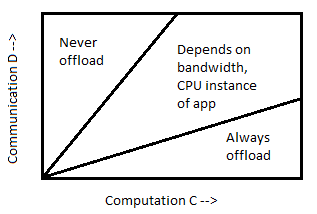
\includegraphics[width=2in]{offload_pic.png}
  \caption{Offloading decision Communication vs Computation}
  \label{fig:offload_pic}
\end{figure}
%%%%%%%%%%%%%%%%%%%%%%%%%%%%%%%%%%%%%%%
\subsection{Offloading Decision Engine}
In this project I have demonstrated some strategies to enrich the offloading decision process with machine learning methods. The decision engine is the mechanism which takes the decision of offloading for the device depending upon `contextual' information of the device such as the bandwidth. \par
\begin{figure}[h]
  \centering
  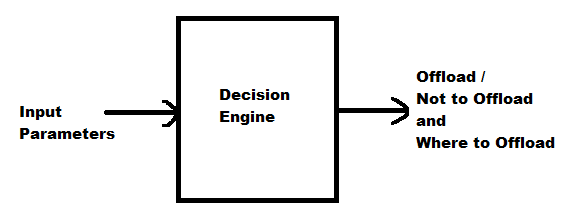
\includegraphics[width=3in]{offload2.png}
  \caption{Offloading Decision Engine}
  \label{fig:offload2}
\end{figure}
Apart from bandwidth other parameters that can be considered are the CPU instance compute intensity(CPU\_low/CPU\_normal/CPU\_high), Data requirement of the application (data\_small/data\_medium/data\_big). \par
In the next section I will discuss the techniques that I have used and then we will study the subsequent results obtained. I have used following methods to create this mechanism:
\begin{itemize}
\item Reinforcement Learning
\item Fuzzy Logic
\item Classification
\end{itemize}
%%%%%%%%%%%%%%%%%%%%%%%%%%%%%%%%%%%%%%%%%%%%%%%%%%%%%%%%%%%%%%%%%%%%%%
\section{Implementation and Results}
In this section I have described all the methods that I have used for the offloading engine mechanism. The Reinforcement learning algorithm is implemented in Python. I have modified the reinforcement learning and neural network code that was provided in the class CS 545 by Dr. Anderson. The fuzzy logic engine is implemented in Java with Android Software Development Kit (SDK). And for classification I have used the same code of Least Squares Classification that was provided in the notebook by Dr. Anderson.
\subsection{Reinforcement Learning}
\subsubsection{The Concept} The objective for any reinforcement learning problem is to
find the sequence of actions that maximizes (or minimizes) the sum
of reinforcements along the sequence.
This is reduced to the objective of acquiring the Q function the
predicts the expected sum of future reinforcements, because the
correct Q function
determines the optimal next action.\par
We have studied in the class that the main objective of Reinforcement learning is to make this approximation as accurate as possible:

    \begin{align*}
      Q(s_t,a_t) \approx \sum_{k=0}^\infty r_{t+k+1}
    \end{align*}

here $s_t$ = state, $a_t$ = actions, and $r_t$ = reinforcements received.
This is usually formulated as the least squares objective:


    \begin{align*}
      \text{Minimize } \mathrm{E} \left ( \sum_{k=0}^\infty r_{t+k+1} - Q(s_t,a_t)\right )^2
    \end{align*}

\subsubsection{The Idea}
Now let's consider the number of battery units consumed by our smartphone as our reinforcements. If we can minimize these units then we achieve reduction in the battery consumption! very intuitive right? \par
We need following things to train the Q function:
\begin{itemize}
   \item action selection
   \item state transitions
   \item reinforcement received
\end{itemize}
The State of the function in our case can have two parameters: Location, Battery Units consumed. The two actions in this mechanism should be Offload, Do Not Offload.\par
We are using Neural Network as our Q function. We will have to evaluate each state and action pair to decide which action to take next. Here is how we train our neural network function:\par
\begin{align*}
nnet = nn.NeuralNetworkQ(ni,nh,output,((p1,p2), (b1,b2), (a1,a2)))
\end{align*}
Here, ni=number of inputs, nh=number of hidden units, output=number of output, p1-p2= range of locations, b1-b2= battery units range, a1,a2=actions to take. \par
Here is some code of the main functions of the implementation:
\begin{small}
\begin{lstlisting}

def initialState():
    position = np.random.randint(1,5)
    processing = np.random.randint(0,2)
    energy_units = 1
    return np.array([position, processing, energy_units])

def reinforcement(s,s1):
    return -1 if(s1[2] > s[2]) else 0

def nextState(s,a):
    s = copy.copy(s)   # s[0] is position, s[1] is velocity. a is -1, 0 or 1
    s[2] = np.random.randint(1,5)
    if (s[1] == 0) :        # Bound next position. If at limits, set velocity to 0.
        s[1] = 1
    elif (s[1] == 1) :
        s[1] = 0
    return s
\end{lstlisting}
\end{small}
In Figure~\ref{fig:offload2} we can see the contour and surface plots of our trained Q function. I am using 5 different locations for the device, with serial numbers 0 to 5. In `Actions' plot we can see the actions taken by the Q function, it shows that it opts to do a local processing(-1) when the device is at locations 0 \& 1; and opts for offloading of processing (1) when at location 2,3 and 4.  
\begin{figure}[h]
  \centering
  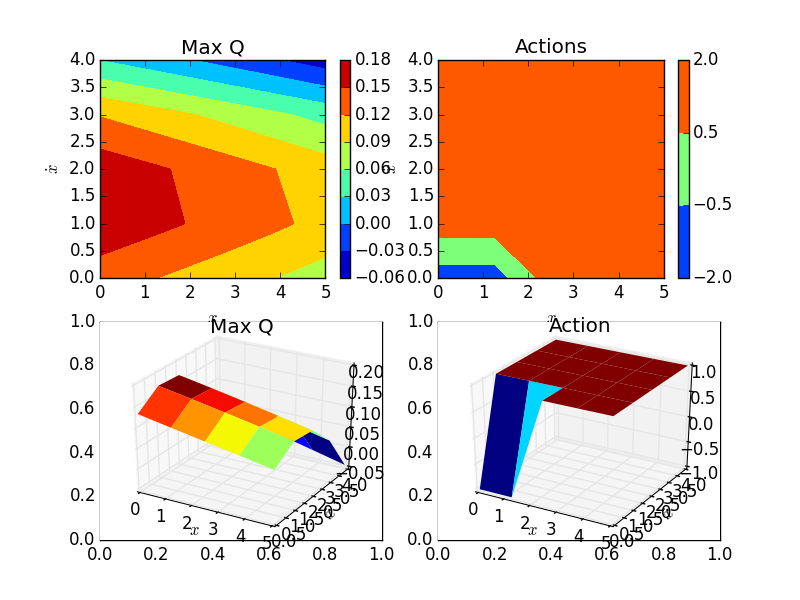
\includegraphics[width=5in]{reinforcement.png}
  \caption{Trained Q function plot}
  \label{fig:offload2}
\end{figure}

%%%%%%%%%%%%%%%%%%%%%%%%%%%%%%%%%%%%%%%
\subsection{Fuzzy Logic Decision Engine}
In this section I have explained the Offloading Decision Engine smartphone app that I have created for an Android device.   
In \cite{flores2013adaptive} the authors have proposed a fuzzy decision engine for code offloading, that considers both mobile and cloud variables. I have implemented a similar engine with relevant parameters and with slightly different rules. 
I have also demonstrated the working of the app. I have used Android Studio platform to develop this app for the Google Nexus 4 smartphone on my Linux machine.

Following are the Fuzzy sets and Some of the rules considered:

\begin{center}
\textbf{\underline{Fuzzy sets considered}}

\begin{itemize}

\item Bandwidth = Speed\_Low, Speed\_Normal, Speed\_High
\item WiFi = available, not available 
\item Data transfered = Data\_Small, Data\_Medium, Data\_Big 
\item CPU instance = CPU\_Low, CPU\_Normal, CPU\_High 


\end{itemize}

\textbf{\underline{Some of the Rules considered}}
\begin{itemize}
\item Remote Processing = Speed\_High AND Data\_Small AND CPU\_Normal
\item Remote Processing = Speed\_Low AND Data\_Small AND CPU\_High
\item Remote Processing = Normal\_Low AND Data\_Small AND CPU\_High
\item Local Processing = Speed\_High AND Data\_Small AND CPU\_Low
\item Local Processing = Speed\_Low AND Data\_Medium AND CPU\_Normal
\item Offload on Local Servers = Remote Processing AND WiFi ON
\item Offload on Remote Servers = Remote Processing AND WiFi OFF
\end{itemize}
\end{center}

Let us see what these parameters define. Bandwidth available to user device can be Low, Normal or High. Data that is used by the application can affect the decision of offloading if the Data is too big the offloading can be expensive. CPU instance required by the application can be Low, Normal and High depending upon the computational requirements of a particular application.
If the WiFi is available to the user then it makes more sense to offload on the local servers rather than the remote servers. So here I am assuming there are multiple locations available with the user where he can offload his application processing and data. After defining these parameters I have assigned grade of truth values to each of the set considered which fuzzy logic uses to classify the outputs.\par
Now let us have a look on the user interface of our offloading app in Figure~\ref{fig:offloading_Local_Server}.
\begin{figure}[h]
  \centering
  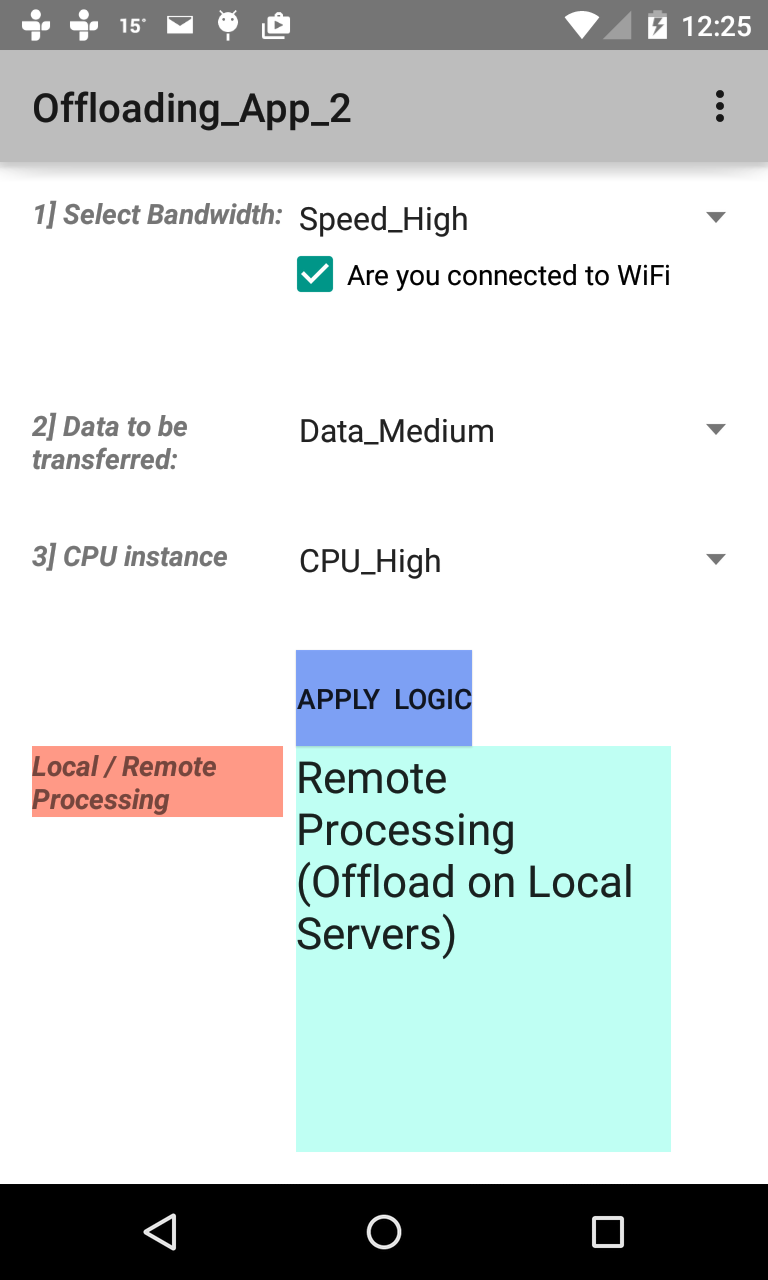
\includegraphics[width=2in]{offloading_Local_Server.png}
  \caption{Offloading Decision Engine}
  \label{fig:offloading_Local_Server}
\end{figure}
As I have said in my current implementation all these parameters are to be filled by user manually. I have created a single screen app where the user can choose from the available options, the Bandwidth available, Data to be transferred, CPU instance requirement of the app, is WiFi available with the user, etc. After giving all these inputs we click on the `APPLY LOGIC' button which can be seen in blue color. The decision of the engine will be seen in the Big Output Box on the right bottom corner.\par
In Figure~\ref{fig:test3png} I have plotted all different parameters that are considered to decide about the processing offloading. The plot for `processing' is the output our decision engine provides. In this plot when the `processing' is at zero the output of the decision engine is `Local Processing', when the processing is at 10000 the output is `Offload on Local Servers', when the processing is at 20000 the output is `Offload on Remote Servers'. The decision of offloading is generally seen when the `CPU instance' is on Higher side and when the `Data' used by the app is on lower side.
\begin{figure}[h!]
  \centering
  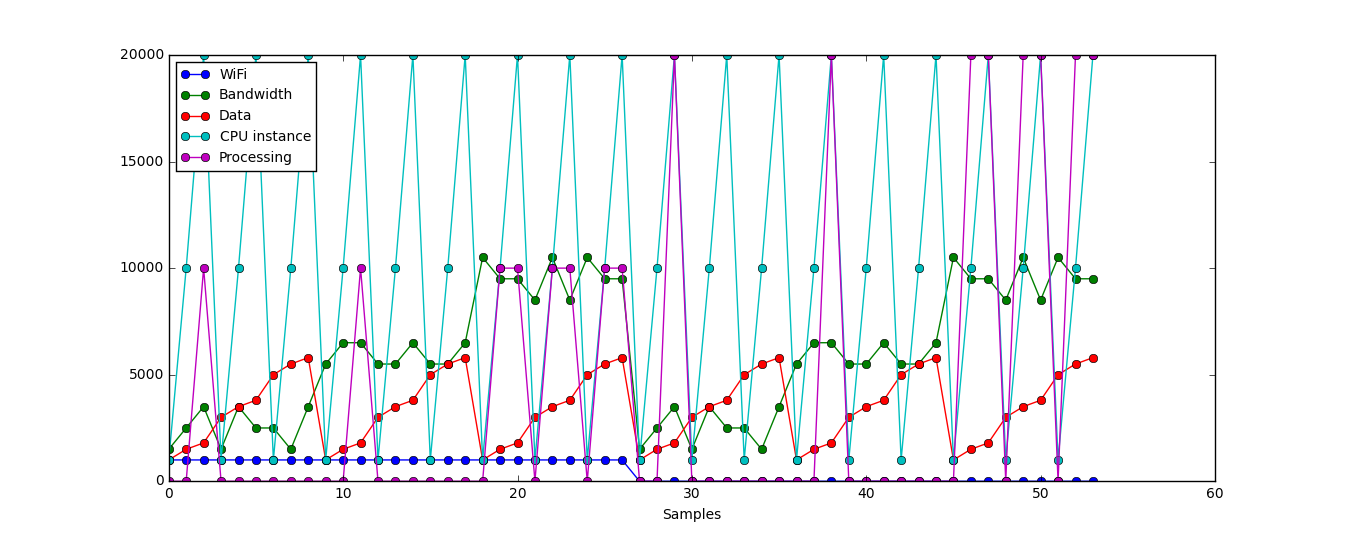
\includegraphics[width=6in]{test3png.png}
  \caption{Offloading Decisions with all parameters}
  \label{fig:test3png}
\end{figure}
\begin{figure}[h!]
  \centering
  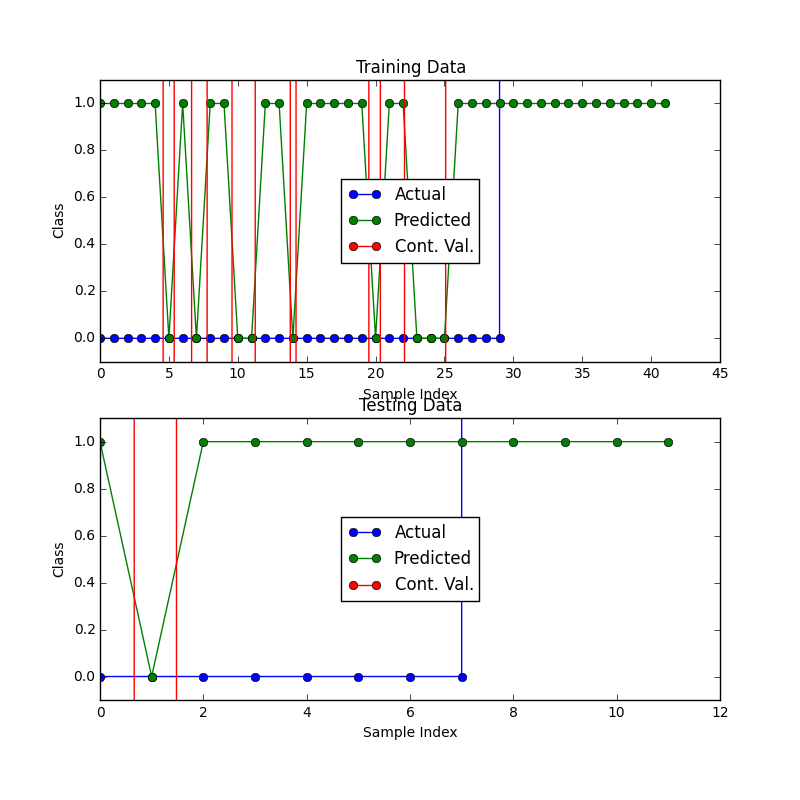
\includegraphics[width=5in]{leastsquares.png}
  \caption{Plot of Least Squares Classifiaction for Training and Testing data \\
Percetage Correct:Training: 56 \% Testing: 20 \%}
  \label{fig:leastsquares}
\end{figure}
%%%%%%%%%%%%%%%%%%%%%%%%%%%%%%%%%%%%%%%
\subsection{Classification}
Finally, I have also tried using classification with Least Squares algorithm. I have created a sample data which looks as follows:
\begin{small}  % to use smaller font for this code.
\begin{lstlisting}
WiFi Bandwidth Data  CPU   Processing
  1    1500      1000  1     0
  0    2500      1500  1     0
  1    3500      1800  2     1
\end{lstlisting}
\end{small}
Here the value WiFi is 1 when it is available and 0 when it is unavailable, values of Bandwidth and Data are in kbs, CPU instance 1 when low and 2 when high, and processing local when value is 0 and remote when value is 1. So we will be predicting the `Processing' column with the help of classification function. 
With some 60 Samples I have divided some data as testing and training data. I have used the code that is provided by Dr. Anderson in the class for the Least Squares algorithm \cite{CS545}.\par
In Figure~\ref{fig:leastsquares} we can see the Actual and predicted values of the offloading decision. 

Because I have very less samples with me I was not able to provide enough training data set, which resulted in poor Percentage of correctness of decision values.
%%%%%%%%%%%%%%%%%%%%%%%%%%%%%%%%%%%%%%%%%%%%%%%%%%%%%%%%%%%%%%%%%%%%%%

\section{Discussion}
For the compute intensive applications the offloading is beneficial. For example if we
want to train a neural network for a smartphone device which has thousands of iterations, we
can offload he training of Q function on the Cloud, and use the trained function for the decision making.\par
Does this make cloud computing the “ultimate” solution to the energy problem for mobile devices? Not
quite. While cloud computing has tremendous potential to save energy, designers must consider several issues including privacy and security, reliability, and handling real-time data\cite{kumar2010cloud}.
%%%%%%%%%%%%%%%%%%%%%%%%%%%%%%%%%%%%%%%%%%%%%%%%%%%%%%%%%%%%%%%%%%%%%%

\section{Conclusion}
Machine learning techniques can be really useful for the smartphone applications. The offloading domain research can benefit from classification or reinforcement learning. I have demonstrated some ways with which we can enhance the offloading process with the help
of an offloading engine which uses machine learning techniques. I found Reinforcement learning is very exciting and promising when used in intuitive situations such as the one which is presented in this project where we can save battery power. We can get good results with the classification algorithms as well when we have large training data set available with us. \par
The main obstacle while using machine learning for the smartphone devices can be to achieve real time processing for the dynamic applications. When the neural network needs a lot of processing to train itself at that time the smartphone-cloud coupling can prove useful as the device need not bother about big number of iterations, it can just offload the processing on cloud. 

%%%%%%%%%%%%%%%%%%%%%%%%%%%%%%%%%%%%%%%%%%%%%%%%%%%%%%%%%%%%%%%%%%%%%%

\bibliographystyle{plainnat}  % or plain, or many other possibilities
\bibliography{cs545_project.bib}


\end{document}
